\chapter{Defining the problem}
This chapter will determine how the further work on the protocol will be handled, by defining how to describe the problem using mathematics. 
By expanding on the definition and the problem statement, a number of system requirements will be defined which must be at least partially satistfied to solve the overall problem.

\section{Development Plan \& Problem Exploration}\label{chp:Problems}
Networks can be described as graphs using graph theory. 
In the case of the protocol the edges are essential for the problem as these represent the available communication.
As the tests in \myref[name]{sec:hardware_tests} have shown, not all sent packages are guaranteed to arrive; hence a weight is given to each edge with a value between 0 and 1.
These weights represents the probability of a given package being received.
This yields a weighted directed graph $G = (V, E, w)$, where $V$ is the set of devices as vertices $v$, $E$ is the set of communication paths as edges $e(v_i, v_j)$, and $w$ is the weight function representing the reliability of any communication path written as $w(v_i,v_j)$.
An example of this can be seen on \myref{fig:network}.

In \myref{fig:examplenetworkgraphs} the two different network types are modelled as graphs; 
\myref{fig:ccrcnetworkgraph} is an example of a \emph{completely connected graph} where every vertex has a direct edge to every other vertex.
\myref{fig:network} is an example of a \emph{strongly connected graph} which is defined in \myref{SCUC}.

\begin{figure}[H]
    \footnotesize
    \begin{subfigure}{0.5\linewidth}
        \centering
        \begin{tikzpicture} [
        node distance = 1 cm, 
        vertex/.style = {circle, draw, fill=blue!10}, 
        label/.style={fill=white}
    ]

    \node[draw=none](0){};
    \node[vertex, left  = 2cm of 0]   (1) {$v_1$};
    \node[vertex, above =     of 0]   (2) {$v_2$};
    \node[vertex, right = 2cm of 0]   (3) {$v_3$};
    \node[vertex, below =     of 0]   (4) {$v_4$};
    
    \path[thick] (1) edge (2) edge (3) edge (4);
    \path[thick] (3) edge (2) edge (4);
    \path[thick] (2) edge (4);
\end{tikzpicture}  
        \caption{Completely connected network.}
        \label{fig:ccrcnetworkgraph}
    \end{subfigure}\hfill
    \begin{subfigure}{0.5\linewidth}
        \centering
        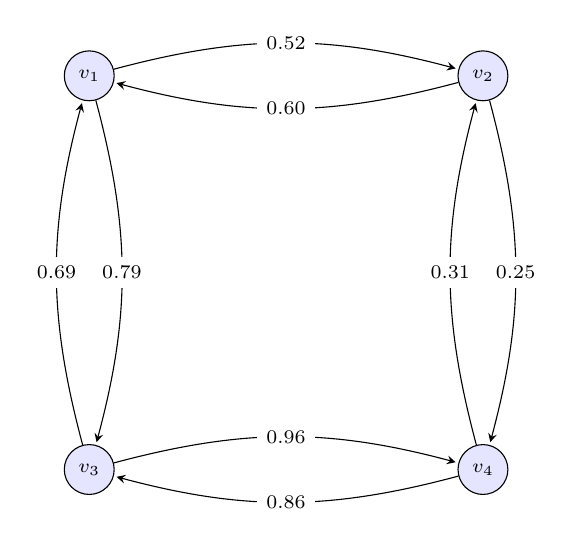
\begin{tikzpicture} [
        node distance = 5 cm, 
        font=\scriptsize, 
        vertex/.style = {circle, draw, fill=blue!10}, 
        edge/.style = {draw, -stealth, shorten >= 1pt},
        label/.style={fill=white}
    ]

    \node[vertex](1){$v_1$};
    \node[vertex, right of=1](2){$v_2$};
    \node[vertex, below of=1](3){$v_3$};
    \node[vertex, below of=2](4){$v_4$};
    
    \path[edge] (1) edge[bend left=15] node [label] {0.79} (3) edge[bend left=15] node [label] {0.52} (2);
    \path[edge] (2) edge[bend left=15] node [label] {0.25} (4) edge[bend left=15] node [label] {0.60} (1);
    \path[edge] (3) edge[bend left=15] node [label] {0.96} (4) edge[bend left=15] node [label] {0.69} (1);
    \path[edge] (4) edge[bend left=15] node [label] {0.31} (2) edge[bend left=15] node [label] {0.86} (3);;
    
\end{tikzpicture}
        \caption{Strongly connected unreliable network with probabilities.}
        \label{fig:network}
    \end{subfigure}
    \caption{Examples of networks modelled as graphs.}
    \label{fig:examplenetworkgraphs}
    \vspace{-20pt}
\end{figure}

\noindent
Creating a protocol for networks as shown in \myref{fig:network} is a complex problem to solve and many issues will become apparent throughout analysis of the problem.
In order to simplify the problem some assumptions are made about the network.

During development of the system, the system could be set up to give \textasciitilde100~\% probability of successfully receiving the message, by wiring the Arduinos together instead of using radio communication; this gives more room to work on the baseline communication issues without having to consider the unreliability of the radio frequency modules.

For this project only networks which can be depicted as completely (as in \myref{fig:ccrcnetworkgraph}) or strongly connected graphs (as in \myref{fig:network}) will be considered, to ensure that all devices will have the possibility to exchange information with every other device.
As a consequence of this, four sub problems will be considered and modelled as graphs.

\bigskip

\noindent The \gls{ccrc}-problem describes a network where all vertices are directly connected with each other, creating a completely connected graph.
All the weights of the edges in this graph are 1, which means that all transmissions are guarenteed to be received. 	

\begin{definition}
	The \acrshort{ccrc}-problem:
	\begin{align*}
		\text{for all } \{v_i, v_j\} \text{ in } V \text{ where } v_i \neq v_j \text{exists a unique edge } e(v_i, v_j) \text{ in } E\\
		\text{where } w(v_i, v_j) = 1
	\end{align*}
\end{definition}

\noindent The \gls{ccuc}-problem describes a completely connected graph however in this scenario there is not a guarrentee that the transmission will be received; all vertices are still in range of each-other.

\begin{definition}
	The \acrshort{ccuc}-problem:
	\begin{align*}
		\text{for all } \{v_i, v_j\} \text{ in } V \text{ where } v_i \neq v_j \text{exists a unique edge } e(v_i, v_j) \text{ in } E\\
		\text{where } w(v_i, v_j) \in\ ]0, 1]
	\end{align*}
\end{definition} 

\noindent The \gls{scrc}-problem describes a \\*strongly connected network meaning at least one vertex does not have direct connections to all other verticies, i.e. there still exists a path from every vertex to every other vertex but at least one pair of vertices requires one or more mediating vertices. 
In this example communication is once again reliable such that all transmissions will be received. 

\begin{definition}
	The \acrshort{scrc}-problem:
	\begin{align*}
		\text{for all } \{v_i, v_j\} \text{ in } V \text{ where } v_i \neq v_j \text{ there is a directed path from } v_i \text{ to } v_j\\
		\text{ and for all edges } e(v_{q}, v_{r}) \text{ in E } w(v_{q}, v_{r}) = 1
	\end{align*}
\end{definition}

\noindent The \gls{scuc}-problem describes the most realistic scenario, a strongly connected network with a chance of not receiving transmissions. 

\begin{definition}\label{SCUC}
	The \acrshort{scuc}-problem:
	\begin{align*}
		\text{for all } \{v_i, v_j\} \text{ in } V \text{ where } v_i \neq v_j \text{ there is a directed path from } v_i \text{ to } v_j\\
		\text{ and for all edges } e(v_{q}, v_{r}) \text{ in E } w(v_{q}, v_{r}) \in\ ]0,1]
	\end{align*}
\end{definition}

\bigskip 
\noindent
The \gls{ccrc}-problem is is the obvious choice for the first iteration, since this is the simplest problem, which requires the least amount of design choices to be fulfilled.
The decision of which problem should follow \gls{ccrc}-solution, is however a more complex discussion.
One could argue for expanding into a still reliable but now only \acrlong{scrc}, as well as arguing for expanding into a unreliably but still \acrlong{ccuc}.
Therefor the chosen order will simply reflect our estimation of which problems will require the least amount of modification.

Another possibility would be to only split the sub problems into three, e.g. \gls{ccrc} $\rightarrow$ \gls{ccuc} $\rightarrow$ \gls{scuc}.
However we deem that a more optimal solution can be derived by working with the strongly connected problem followed by the unreliable problem and then combine the solutions to solve the \gls{scuc}-problem.

In addition to these four sub problems, some more practical problems will be abstracted away for in the first iteration.
An example of such a abstraction could be starting multiple devices at the same time.
Solutions to these practical problems will be implemented continually during the development. 
This approach increases the probability of having a working solution at the end of this project without over- or underestimating the workload. 
